\documentclass[12pt]{article}
\usepackage[utf8]{inputenc}
\usepackage{amsmath, amssymb}
\usepackage{xcolor}
\usepackage{geometry}
\usepackage{hyperref}
\usepackage{fancyhdr}
\usepackage{enumitem}
\usepackage{minted} % Code highlighting
\usepackage{booktabs} % Clean tables
\usepackage{tikz} % Optional for concept maps

\geometry{margin=1in}
\hypersetup{colorlinks=true, linkcolor=blue, urlcolor=cyan}

\pagestyle{fancy}
\fancyhf{}
\fancyhead[L]{\textbf{\TOPICTITLE}}
\fancyhead[R]{\thepage}

% -------------------------------
% Topic Metadata
% -------------------------------
\newcommand{\TOPICTITLE}{Transport Layer}
\title{\TOPICTITLE\\\large Study-Ready Notes}
\author{Compiled by Andrew Photinakis}
\date{\today}

\setlength{\headheight}{15pt}

\begin{document}
\maketitle
\tableofcontents
\newpage

% This LaTeX file should be saved at: computer_networks/transport_layer/transport_layer_introduction.tex

\section{Introduction to Transport Layer Services}

\begin{itemize}
    \item Transport layer provides logical communication between application processes running on different hosts
    \item Key services include:
          \begin{itemize}
              \item Multiplexing and demultiplexing
              \item Connectionless transport: UDP
              \item Principles of reliable data transfer
              \item Connection-oriented transport: TCP
              \item Principles of congestion control
              \item TCP congestion control
              \item Evolution of transport-layer functionality
          \end{itemize}
\end{itemize}

\textcolor{blue}{[Summary: The transport layer enables communication between application processes across networks, providing essential services like multiplexing, reliable data transfer, and congestion control through protocols like TCP and UDP.]}

\section{Transport Layer Overview}

\subsection{Learning Objectives}
\begin{itemize}
    \item Understand principles behind transport layer services:
          \begin{itemize}
              \item Multiplexing and demultiplexing
              \item Reliable data transfer
              \item Flow control
              \item Congestion control
          \end{itemize}
    \item Learn about Internet transport layer protocols:
          \begin{itemize}
              \item UDP: connectionless transport
              \item TCP: connection-oriented reliable transport
              \item TCP congestion control
          \end{itemize}
\end{itemize}

\section{Transport Services and Protocols}

\subsection{Core Functions}
\begin{itemize}
    \item Provides \textbf{logical communication} between application processes running on different hosts
    \item Transport protocols actions in end systems:
          \begin{itemize}
              \item \textbf{Sender}: breaks application messages into \textbf{segments}, passes to network layer
              \item \textbf{Receiver}: reassembles segments into messages, passes to application layer
          \end{itemize}
    \item Two transport protocols available to Internet applications:
          \begin{itemize}
              \item \textbf{TCP} (Transmission Control Protocol)
              \item \textbf{UDP} (User Datagram Protocol)
          \end{itemize}
\end{itemize}

\subsection{Network Architecture Context}
\begin{figure}[h]
    \centering
    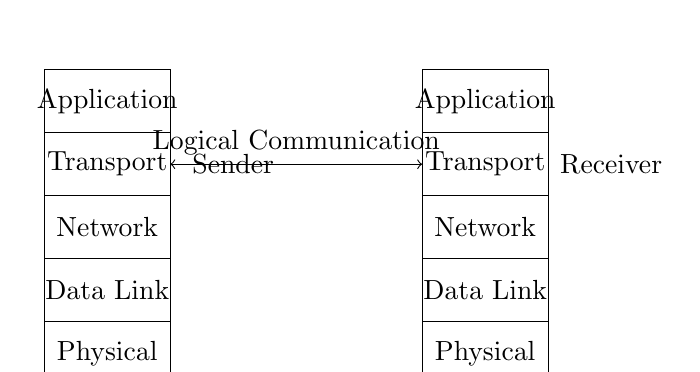
\begin{tikzpicture}[scale=0.8]
        \draw (0,0) rectangle (2,1) node[midway] {Application};
        \draw (0,-1) rectangle (2,0) node[midway] {Transport};
        \draw (0,-2) rectangle (2,-1) node[midway] {Network};
        \draw (0,-3) rectangle (2,-2) node[midway] {Data Link};
        \draw (0,-4) rectangle (2,-3) node[midway] {Physical};
        \node at (3,-0.5) {Sender};

        \draw (6,0) rectangle (8,1) node[midway] {Application};
        \draw (6,-1) rectangle (8,0) node[midway] {Transport};
        \draw (6,-2) rectangle (8,-1) node[midway] {Network};
        \draw (6,-3) rectangle (8,-2) node[midway] {Data Link};
        \draw (6,-4) rectangle (8,-3) node[midway] {Physical};
        \node at (9,-0.5) {Receiver};

        \draw[<->] (2,-0.5) -- (6,-0.5) node[midway,above] {Logical Communication};
    \end{tikzpicture}
    \caption{Transport layer in network protocol stack}
    \label{fig:protocol_stack}
\end{figure}

\textcolor{blue}{[Summary: Transport protocols operate at end systems, segmenting application messages for transmission and reassembling them upon receipt, with TCP and UDP as the primary Internet protocols.]}

\section{Transport vs. Network Layer Services}

\subsection{Household Analogy}
\begin{itemize}
    \item \textbf{Hosts} = houses
    \item \textbf{Processes} = kids
    \item \textbf{Application messages} = letters in envelopes
    \item 12 kids in Ann's house sending letters to 12 kids in Bill's house
\end{itemize}

\subsection{Layer Responsibilities}
\begin{itemize}
    \item \textbf{Network layer}: logical communication between hosts
    \item \textbf{Transport layer}: logical communication between processes
    \item Transport layer relies on and enhances network layer services
\end{itemize}

\begin{table}[h]
    \centering
    \begin{tabular}{p{0.45\textwidth}p{0.45\textwidth}}
        \toprule
        \textbf{Network Layer}              & \textbf{Transport Layer}                           \\
        \midrule
        Host-to-host communication          & Process-to-process communication                   \\
        Logical communication between hosts & Logical communication between processes            \\
        Provides basic datagram delivery    & Enhances delivery with reliability, ordering, etc. \\
        \bottomrule
    \end{tabular}
    \caption{Comparison of Network vs. Transport Layer Services}
    \label{tab:network_vs_transport}
\end{table}

\textcolor{orange}{[Mnemonic: "Houses Host, Kids Process" - Network layer connects houses (hosts), Transport layer connects kids (processes) within houses.]}

\section{Transport Layer Actions}

\subsection{Sender Operations}
\begin{enumerate}
    \item Receives application-layer message
    \item Determines segment header field values
    \item Creates segment with header and payload
    \item Passes segment to IP (network layer)
\end{enumerate}

\begin{figure}[h]
    \centering
    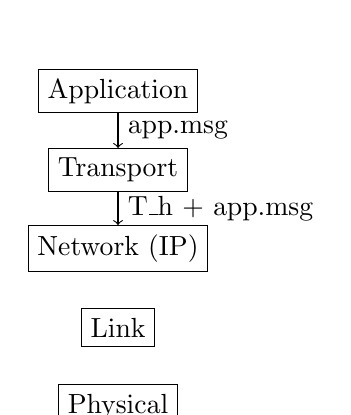
\begin{tikzpicture}
        \node[draw, rectangle] (app) at (0,2) {Application};
        \node[draw, rectangle] (trans) at (0,1) {Transport};
        \node[draw, rectangle] (net) at (0,0) {Network (IP)};
        \node[draw, rectangle] (link) at (0,-1) {Link};
        \node[draw, rectangle] (phys) at (0,-2) {Physical};

        \draw[->] (app) -- (trans) node[midway,right] {app.msg};
        \draw[->] (trans) -- (net) node[midway,right] {T\_h + app.msg};
    \end{tikzpicture}
    \caption{Sender-side transport layer processing}
    \label{fig:sender_processing}
\end{figure}

\subsection{Receiver Operations}
\begin{enumerate}
    \item Receives segment from IP (network layer)
    \item Checks header values for correctness
    \item Extracts application-layer message from segment
    \item Demultiplexes message up to application via appropriate socket
\end{enumerate}

\begin{figure}[h]
    \centering
    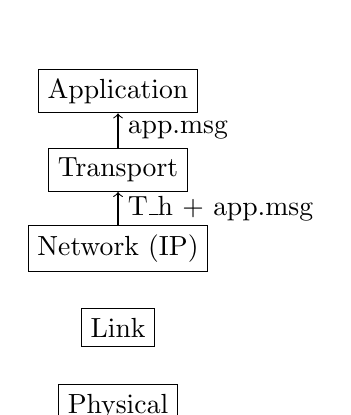
\begin{tikzpicture}
        \node[draw, rectangle] (app) at (0,2) {Application};
        \node[draw, rectangle] (trans) at (0,1) {Transport};
        \node[draw, rectangle] (net) at (0,0) {Network (IP)};
        \node[draw, rectangle] (link) at (0,-1) {Link};
        \node[draw, rectangle] (phys) at (0,-2) {Physical};

        \draw[->] (net) -- (trans) node[midway,right] {T\_h + app.msg};
        \draw[->] (trans) -- (app) node[midway,right] {app.msg};
    \end{tikzpicture}
    \caption{Receiver-side transport layer processing}
    \label{fig:receiver_processing}
\end{figure}

\textcolor{blue}{[Summary: The transport layer segments application data at the sender and reassembles it at the receiver, handling header processing and message demultiplexing to the correct application process.]}

\section{Internet Transport Protocols}

\subsection{TCP: Transmission Control Protocol}
\begin{itemize}
    \item \textbf{Reliable, in-order delivery}: Ensures all data arrives correctly and in sequence
    \item \textbf{Congestion control}: Prevents network overload by adjusting transmission rate
    \item \textbf{Flow control}: Prevents overwhelming the receiver
    \item \textbf{Connection setup}: Requires establishment of connection before data transfer
\end{itemize}

\subsection{UDP: User Datagram Protocol}
\begin{itemize}
    \item \textbf{Unreliable, unordered delivery}: No guarantees on delivery or ordering
    \item \textbf{No-frills extension of "best-effort" IP}: Minimal overhead beyond IP
    \item \textbf{Services not available}:
          \begin{itemize}
              \item Delay guarantees
              \item Bandwidth guarantees
          \end{itemize}
\end{itemize}

\begin{table}[h]
    \centering
    \begin{tabular}{p{0.4\textwidth}p{0.5\textwidth}}
        \toprule
        \textbf{TCP Features}                         & \textbf{UDP Features}                    \\
        \midrule
        Connection-oriented                           & Connectionless                           \\
        Reliable delivery                             & Best-effort delivery                     \\
        In-order delivery                             & No ordering guarantees                   \\
        Flow control                                  & No flow control                          \\
        Congestion control                            & No congestion control                    \\
        Higher overhead                               & Lower overhead                           \\
        \textbf{Use cases}: Web, email, file transfer & \textbf{Use cases}: DNS, VoIP, streaming \\
        \bottomrule
    \end{tabular}
    \caption{Comparison of TCP vs. UDP Protocols}
    \label{tab:tcp_vs_udp}
\end{table}

\textcolor{teal}{[Concept Map: Transport Layer → TCP (reliable, connection-oriented, flow/congestion control) vs UDP (unreliable, connectionless, minimal overhead) → Applications choose based on reliability vs performance needs.]}

\section{Study Aids and Exam Preparation}

\subsection{Key Concepts}
\begin{itemize}
    \item Understand the difference between network layer (host-to-host) and transport layer (process-to-process) communication
    \item Memorize the characteristics and use cases for TCP vs UDP
    \item Be able to describe the segmentation process at sender and reassembly at receiver
    \item Know the household analogy for understanding layer responsibilities
\end{itemize}

\subsection{Practice Questions}
\begin{enumerate}
    \item \textbf{Compare and contrast} the services provided by TCP and UDP. When would you choose one over the other?

    \item Describe the process of \textbf{multiplexing and demultiplexing} at the transport layer. How does the transport layer ensure messages reach the correct application process?

    \item Explain the \textbf{household analogy} for understanding the difference between network and transport layer services.

    \item What are the key \textbf{transport layer actions} performed by the sender and receiver during data transmission?

    \item Why is \textbf{congestion control} an important transport layer function, and which protocol provides it?
\end{enumerate}

\textcolor{orange}{[Mnemonic: "TCP: Reliable Connection, UDP: Unreliable Datagram" - TCP establishes reliable connections while UDP sends unreliable datagrams.]}

\end{document}